
\chapter{Introduction}\label{C:intro}

% Shorterned form of your dreams and aspirations
% may want to include some stuff about github and refactoring here as is 
% speaks about how mecessay it is to have a good merge
According to Bertino \cite{Bertino2012} \emph{Version control systems} provide a way of allowing multiple developer to collaborate. When multiple developers work on the same source code there is a risk that they have conflicting changes for the same portion of the source code.  One way of managing these conflicting changes is by ensuring only one person can edit a file at a time. This locking mechanism was recommend by Tichy \cite{Tichy1982} for the RCS version control system. The problem with this is that one person stops other people from being able to edit the file. An alternative approach is to allow multiple changes to a file and to automatically resolve most of them in a process called a \emph{merge}.  The merge process compares the changes made for one version with the changes made on the other revision. If the merge process determines that changes can coexist it creates a merged file that contains all the changes. The changes that cannot be automaticaly merged are known as \emph{merge conflicts}.  The merge conflicts need to be manually checked and edited to make a merged file with the correct changes.

\begin{figure}[h]
 \begin{center}
 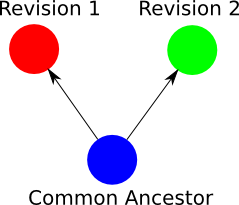
\includegraphics[scale=1]{introRevisions}
 \end{center}
 \caption{A file that has two different revisions}
 \label{fig:introRevisions}
\end{figure}


Internally the merge process need to determines what changes have happened to both of the revisions being compared.   In figure  ~\ref{fig:introRevisions} there are two revision that are derived from a common ancestor. It is possible to determine what has been deleted, inserted or changed by comparing each of the revisions against the common ancestor.  This is often done as a linear comparision which work very well when there has been no change in the order.

% Internally the merge process need to determines what changes have happened 
% to both of the revisions being compared.  One way of doing this is by 
% comparing both revisions with a common ancestor to find any differences. An 
% algorithm that resolves \emph{the longest common subsequence}(LCS) is often 
% used to compare the differences between the common ancestor and the revision 
% we are interested in.  A LCS contains the longest set of identical items for 
% both versions that are in the same order.

% LCS algorithm does not detect when there is a change in the order such as 
% when blocks of source code have been swapped. This is an issue because it is 
% possible for a program to behave in the same manner even when source code is 
% in a different order.
% The swapping of the order of the method is still counted by LCS algorithms 
% as being a change in the code even though both programs .

However, if there has been a change where a block of source code has been moved from one place to another a linear comparison instead determines that two changes have occured.  This is equivalent to deleting a block of source code in the common ancestor and inserting that source code elsewhere. This becomes an issue because it is possible for a program to behave in the same manner even when source code is in a different order.  An example of this is if a Java programmer changes the order of methods within a program.  The program will behave in the same way as changing the order of methods does not change any functionality, however the source code is now different. The swapping of the order of the method is still counted as being two different changes even though the program could behave in the same manner as it did before the change took place.

Without any further analaysis this unnecessary change is recorded in the merged file.  Although there has been no functional change the version control systems will treat the relocation of blocks of source code exactly like a change in functionality.  Whenever a programmer attempts to update their code to incorporate any change in functionality, the change to the order of methods is also made to their code.  If a programmer is already familiar with the old structure of code changing it unnecessarily could be disconcerting.   

If two different changes in the order of methods occur, one for each revision, it is possible to get a merge conflict in spite of the revisions being functionally equivalent.

This thesis explores a way of allowing a version source control system to detect when the source code has been reordered.  It also introduces the concept of maintaining multiple seperate views of differently ordered but equivalent source code for the purpose of reducing the number of changes introduced in a merge. 
 
In order to do this the source code needs to be divided into understandable sections. When each of these sections for each revising are compared it is possible to determine if a section has been moved.  This enhances what can be detected when examining the differences between two files.



